\subsection{SHM and RDMA Ring Buffer}
\label{subsec:lockless-queue}

\iffalse
\begin{figure}[t]
	\centering
	
\includegraphics[width=0.4\textwidth]{images/fixme.pdf}
	\vspace{-5pt}
	\caption{Performance comparison of queues.}
	\label{fig:queue-performance}
\end{figure}
\fi

\begin{figure}[t]
	\centering
	\subfloat[Traditional.]{
		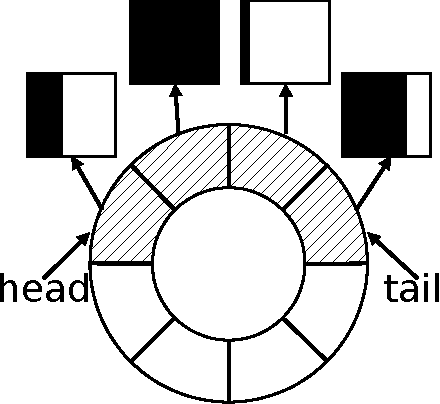
\includegraphics[width=0.15\textwidth]{images/ringbuffer_traditional}
		\label{fig:ringbuffer-traditional}
	}
	\hspace{0.02\textwidth}
	\subfloat[\sys.]{
		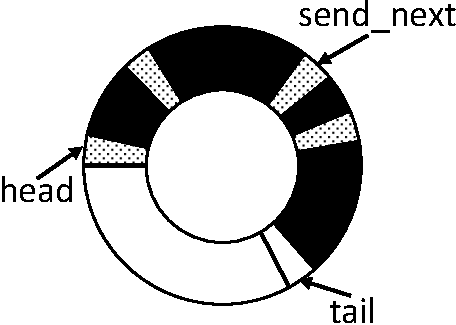
\includegraphics[width=0.16\textwidth]{images/ringbuffer_new}
		\label{fig:ringbuffer-new}
	}
	\vspace{-10pt}
	\caption{Ring buffer data structures. Shaded part is packet metadata, and black part is payload.}
\end{figure}

\RED{Need a performance comparison figure of ring buffer architectures.}

Traditionally, the network stack send and receive packets from NICs using a ring buffer.
As Figure~\ref{fig:ringbuffer-traditional} shows, it leads to buffer management overhead and internal fragmentation.
Traditional NICs support a limited number of ring buffers, so multiple connections may multiplex through one ring buffer, and this design enables moving payload to per-connection buffers without copy.
Fortunately, RDMA write verbs open up new design possibility.
Our innovation is to have \emph{one ring buffer per socket connection} and store packets back-to-back, as Figure~\ref{fig:ringbuffer-new} shows.
The sender determines the ring buffer and offset (i.e. \emph{tail} pointer), then use RDMA write verb to send the packet to the tail pointer.
During sending, the receiver CPU does not need to do anything.
When the receiver application calls \texttt{recv}, data is dequeued from the \emph{head} pointer.
The process is similar for SHM because both SHM and RDMA support write primitives.

%%We first revisit requirements of the queue between a pair of communicating threads in different applications or hosts. A sender enqueues messages sequentially. At the same time, a receiver peeks and dequeues messages at any position. The message may be a control command or data of a FD, so the message size is variable.
%%Our aim is high throughput and low latency when messages in the queue are dequeued in the same order as enqueued, and preserve liveness when dequeuing in arbitrary order.
%SHM and RDMA are state-of-the-art methods for intra-host and inter-host communication respectively.
%%As Figure~\ref{fig:queue-performance} shows, 
%Sharing \emph{head} and \emph{tail} pointers between sender and receiver introduces inter-core cache migration overheads in shared memory and unacceptable latency for RDMA.
%For high throughput and low latency, our principle is that each shared memory region is either writable by the sender or receiver, but never both.
%So we keep \textit{head} and \textit{tail} pointers locally in sender and receiver respectively.
%Because the receiver needs to modify \emph{isdel} and \emph{nextptr} fields, we create a \emph{shadow ring buffer} in receiver's private memory and update the corresponding offset in place of shared memory.

%Most ring buffer designs share \textit{head} and \textit{tail} pointers between sender and receiver, which introduces an additional cache migration or RDMA operation. To eliminate such overhead, we keep \textit{head} and \textit{tail} pointers locally in sender and receiver respectively.
To tell whether the ring buffer is full, the sender maintains a \textit{queue credits} count, indicating the number of free bytes in ring buffer.
%Many applications use the limited send buffer as a back-pressure signal to control how much data to generate.
%To achieve fair queue utilization among FDs, the sender also maintains \emph{per-FD credits}.
When sender enqueues a packet, it consumes credits. When receiver dequeues a message, it increments a counter locally, and writes a \textit{credit return flag} in sender's memory once the counter exceeds half the size of ring buffer. The sender regains queue credits upon detecting the flag.
%Notice that this mechanism is irrelevant to congestion control; the latter is handled by the NIC hardware~\cite{zhu2015congestion}.

\parab{Two copies of ring buffers on send and receive sides.}
The above mechanism still incurs buffer management on the send side because the sender needs to construct RDMA message in a buffer.
Second, it does not support container live migration because the remaining data in RDMA queue is hard to migrate.
Third, we aim to batch small messages to improve throughput.
To this end, we maintain a copy of ring buffers on both send and receive sides.
The sender side writes its local ring buffer, and invokes RDMA to synchronize the sender to the receiver.
We use an RDMA RC QP for each ring buffer, and maintain a counter of in-flight RDMA messages.
If the counter does not exceed threshold, an RDMA message is sent for every socket \texttt{send} operation.
Otherwise, the message is not sent, and \emph{send\_next} marks the first unsent message.
Upon completion of an RDMA write, we send a large message containing all unsent changes (\emph{send\_next} to \emph{tail} in Figure~\ref{fig:ringbuffer-new}).
This adaptive batching mechanism minimizes latency on idle links and maximizes throughput on busy links.
For SHM, we have only one copy of ring buffer shared by two processes, and synchronization is done by cache coherence hardware.

%Before sending, sender clears header of the next message to prevent the receiver from considering junk data in the ring buffer to be a message. Next, sender writes payload, then writes header, finally advances \textit{tail}. Receiver polls \textit{isvalid} at \textit{head} pointer, then copies the message, finally advances \textit{head}.
%For RDMA, the sender maintains a local copy of ring buffer, and we use one-sided RDMA write to synchronize updates from sender to receiver.
%For RDMA, it is known that one-sided verbs has higher throughput than two-sided ones; short messages has lower throughput than large ones~\cite{kalia2014using,kaminsky2016design}.
%In light of this, the inter-host queue has two identical copies in pinned sender and receiver memory, and we use one-sided RDMA write to synchronize updates from sender to receiver.
%\libipc{} polls CQ to limit the number of in-flight (sent but not acknowledged) messages, which is not only required by RDMA NIC, but also enables \emph{adapative batching}~\cite{li2016clicknp,li2017kv}.
%When a message is enqueued to the ring buffer and the RDMA send queue is not full, it is immediately sent as an RDMA message.
%When \libipc{} polls CQ and finds an empty slot in send queue, it sends all queued but unsent data in queue as an RDMA message, because the messages are stored back-to-back in the queue.


\parab{Consistency between payload and metadata.}
%One may believe that out-of-order execution in CPU may mandate the use of memory fence instructions. 
%For shared-memory queue, 
For SHM, X86 processors from Intel and AMD provide total store ordering~\cite{sewell2010x86,intel-manual}, which implies that two writes are observed by other cores in the same order as they were written. An 8-byte \texttt{MOV} instruction is atomic, so writing a header is atomic. Because sender writes header after payload, the receiver would read a consistent message. Therefore, memory fence instruction is unnecessary.

Because RDMA does not ensure write ordering within a message~\cite{infiniband2000infiniband}, we do need to make sure a message is completely arrived. Sender uses \textit{RDMA write with immediate} verb to generate completions on receiver. The receiver polls RDMA completion queue rather than the ring buffer. RDMA ensures cache consistency on receiver, and the completion is guaranteed to be delivered after writing the data.


\parab{Amortize polling overhead.}
Polling ring buffers wastes CPU cycles of the receiver when a pair of threads do not communicate frequently. We amortize polling overhead using two techniques.
First, for RDMA queues, we leverage the RDMA NIC to multiplex event notifications into a single queue.
Each thread uses a \emph{shared completion queue} for all RDMA connections, so it only needs to poll one queue rather than multiple queues.

Second, each queue can switch between \textit{polling} and \textit{interrupt} modes. The queue to the monitor is always in polling mode. Receiver of each queue maintains a counter of consecutive empty polls. When it exceeds a threshold, the receiver sends a message to sender notifying that the queue is entering interrupt mode, and stops polling after a short period. When sender writes to a queue in interrupt mode, it also notifies the monitor and the monitor will signal the receiver to resume polling.


\subsection{Zero Copy}
\label{subsec:zerocopy}

\begin{figure}[t]
	\centering
	\subfloat[Intra-server SHM. 1) Get physical page and set copy-on-write; 2) send page address via SHM; 3) map received page; 4) (optional) remap when sender write / memcpy / recv.]{
		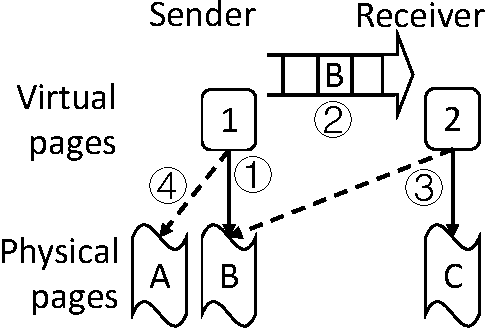
\includegraphics[width=0.22\textwidth]{images/zerocopy_intra}
		\label{fig:zerocopy-intra}
	}
	\hspace{0.02\textwidth}
	\subfloat[Inter-server RDMA. 1) Get physical page and set copy-on-write; 2) get free page from pool; 3) send data via RDMA; 4) send page address via RDMA; 5) map received page; 6) return unmapped page to pool.]{
		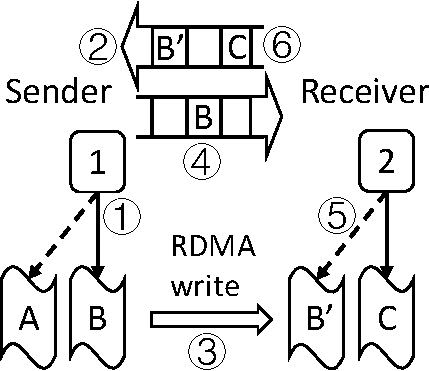
\includegraphics[width=0.21\textwidth]{images/zerocopy_inter}
		\label{fig:zerocopy-inter}
	}
	\vspace{-10pt}
	\caption{Procedure to send a page with zero copy.}
\end{figure}


\RED{Need a performance comparison figure for copy, batch page remapping, single page remapping, etc.}

As Sec.~\ref{subsec:per-byte-overhead} discussed, the main challenge for zero copy is to maintain the semantics of socket API.
Fortunately, virtual memory provides a layer of indirection, and many works leverage this \emph{page remapping} technique.
%Rather than copying, we can remap the physical pages from sender's virtual addresses to receiver's.
Linux zero copy socket~\cite{linux-zero-copy} only support send side, by setting the data pages as copy-on-write.
However, many applications overwrite the send buffer frequently, so the copy-on-write mechanism simply delays the copy from \texttt{send} time to first overwrite time. 
To achieve zero copy receive, 20 years ago, BSD~\cite{thadani1995efficient} and Solaris~\cite{chu1996zero} remap the virtual page of application buffer to the physical page of system buffer. However, as Table~\ref{tab:operation-performance} shows, on modern CPUs, mapping one page has even higher cost than copying it, because of kernel crossing and TLB flush costs.
Recently, many high performance TCP/IP stacks~\cite{han2012megapipe,yasukata2016stackmap} and socket-to-RDMA libraries~\cite{rsockets,socketsdirect} provide both standard socket API and an alternative zero-copy API, but none of them achieves zero copy for the standard API.
Further, no existing works support zero copy for intra-host sockets.


%A sender may write the send buffer after non-blocking \texttt{send}, and the receiver does not know the receive buffer before \texttt{recv}.
% so we can remap virtual address of a buffer to another physical page if the data occupies entire 4~KiB pages.

To enable zero-copy, we need to modify the NIC driver to expose several kernel functions related to page remapping. 
%Due to the remapping overhead (Table~\ref{tab:operation-performance}), we only use zero-copy for \texttt{send} or \texttt{recv} with at least 8~KiB payload size. Smaller messages are copied instead.
To amortize page remapping cost, we only use zero copy for \texttt{send} or \texttt{recv} with at least 8~KiB payload size.
Smaller messages are copied instead.

\parab{Page alignment.}
Page remapping only works when the send and receive addresses are page aligned and the transfer contains entire pages.
We intercept \texttt{malloc} and \texttt{realloc} functions and allocate 4~KiB aligned addresses for allocations with multiple-of-4K sizes, so most buffers will align to page boundary, while not wasting memory for small allocations.
If the size of sent message is not a multiple of 4~KiB, the last chunk of data is copied on \texttt{send} and \texttt{recv}.

%\parab{Amortize page remapping cost.}


\parab{Minimize copy-on-write.}
%After \texttt{send}, because the application may read the buffer or send the buffer to other receivers, it needs to write-protect the buffer.
%\texttt{recv} also needs to write-protect received buffers.
When sender overwrites the buffer after \texttt{send}, existing designs use copy-on-write. %Copy is required because the sender may read the non-written part of the page.
%Because applications almost always reuse the buffer for subsequent send operations, copy-on-write is invoked in most cases, making zero-copy essentially useless on sender.
Our observation is that most applications do not write send buffers byte-by-byte. Instead, they overwrite entire pages of the send buffer via \texttt{recv} or \texttt{memcpy}, so it is unnecessary to copy original data of the page.
%For \texttt{recv}, the old read-only mapping can be safely discarded.
For \texttt{memcpy}, we invoke the kernel to remap new pages and disables copy-on-write, then do the actual copy.
For \texttt{recv}, the old page mappings are replaced by the received pages.


\parab{Page allocation overhead.}
Page remapping requires the kernel to allocate and free pages for each zero copy \texttt{send} and \texttt{recv}. 
Page allocation in kernel uses a global lock, which is inefficient. \libipc{} manages a pool of free pages in each process locally.
\libipc{} also tracks the origin of received zero-copy pages.
When a page is unmapped, if it is from another process, \libipc{} return the pages to the owner through a message.

\parab{SHM: Send page addresses securely in user space.}
For intra-host socket, we send the physical page addresses in a message in user-space queues, as step 2 in Figure~\ref{fig:zerocopy-intra}.
We must prevent unsolicited remapping of arbitrary pages.
To this end, \libipc{} invokes a modified NIC driver to 
get obfuscated physical page addresses of the send buffer and send the address to receiver via shared memory queue.
On the receiving side, \libipc{} invokes the kernel to remap the obfuscated physical pages to the application-provided receive buffer virtual address.

\parab{Zero Copy under RDMA.}
\libipc{} initializes a pinned page pool on receiver and send the physical addresses of the pages to the sender.
The sender manages the pool.
On sender, \libipc{} %pins the send buffer if it has not been pinned, then 
allocates pages from the remote receiver page pool to determine the remote address of RDMA write, as step 2 in Figure~\ref{fig:zerocopy-inter}.
On receiver, when \texttt{recv} is called, \libipc invokes the NIC driver to map pages in the pool to application buffer virtual address.
After the remapped pages are freed (e.g. overwritten by another \texttt{recv}), \libipc{} returns them to the pool manager in sender (step 6).
%If the OS runs out of memory, \libipc{} unpins pages to reclaim memory.
%For security, kernel validates that page numbers are in the huge-page receive buffer.

%\subsubsection{Zero Copy TCP}
%\label{subsec:zero-copy-tcp}
%
%For TCP connections, we optimize the user-space TCP/IP stack to remove memory copy between \libipc{} and NIC.
%Because the payloads of sent and received packets need to align at 4~KiB page boundary, we leverage scatter-gather support in modern NICs~\cite{mellanox} to separate packet header from application payload.
%%During initialization, \libipc{} queries IP and Ethernet MAC address from the kernel and constructs a packet header template.
%For \texttt{send}, \libipc{} constructs a packet header to a NIC send work request, then fills in the payload buffer address from application. 
%For receiving data, in background, \libipc{} issues NIC receive work requests with a 54-byte buffer to store Ethernet, IPv4 and TCP headers, followed by a page-aligned buffer to store payload.
%%In corner cases where the received header length is not 54 bytes, \libipc{} reassembles the packet.
%Upon \texttt{recv}, the payload buffer is remapped to application.

\subsection{Cooperative Multitasking}
\label{subsec:process-mux}

To deal with the scenario where multiple threads share a CPU core, rather than using OS thread wakeup, we use cooperative multitasking to switch thread contexts efficiently.


\parab{Event notification.}
%To minimize context switch, \sys{} runs in user mode and uses cooperative multitasking to multiplex processes on CPU cores. 
Coordination and delegation based on message passing requires processes to respond to messages promptly. However, processes may execute application code without calling \libipc{} for a long time. To address this issue, we design a \textit{signal} mechanism analogous to interrupts in operating systems. Event initiators  first poll the receive queue for a period of time for ACK. If no reply, it sends a Linux \texttt{signal} to the receptor and wake up the process.

The signal handler, registered by \libipc{}, first determines whether the process is executing application or \libipc{} code. \libipc{} sets and clears a flag at entry and exit of the library. If signal handler finds that the process is in \libipc, it does nothing and \libipc{} will process the event before returning control to the application. Otherwise, the signal handler immediately processes messages from the emergency queue to the monitor, before returning control to the application. 
%Because \libipc{} is designed to be fast and non-blocking, message passing initiators will soon receive the response.

\parab{Polling and sleep.}
When an application calls non-blocking socket operations, \libipc{} polls queues of the specified FD and the emergency queue to the monitor, then returns immediately. For blocking operations (e.g., blocking recv, connect and epoll\_wait), \libipc{} first polls the queues once. If the operation is not completed, \libipc{} calls \texttt{sched\_yield} to yield to other processes on the same core. %As stated in Sec.~\ref{subsec:bottleneck}, context switch in cooperative multitasking only takes 0.4~$\mu$s. However, an application may wait a long time for an external event, making frequent wake-ups wasteful. In this regard, we count consecutive wake-ups which does not process any message, and puts the process to sleep when this reaches a threshold. 
If \libipc{} continues to yield for a certain number of rounds, it will put itself into sleep. Before sleeping, it sends a message to the monitor and all peers, so they can wake it up later through a message.

%\parab{Handling events from kernel.}
%An application often needs to poll kernel FDs (\textit{e.g.} files and semaphores) together with socket FDs.
%\libipc{} creates a per-process \textit{epoll thread} to poll kernel FDs for all application threads. When it receives a kernel event, it broadcasts the event to application threads via shared memory queues.%\texttt{Epoll\_wait} in \libipc{} will return such kernel events in addition to socket events. Note that Linux allows an event to be received by multiple threads sharing the FD.

%\parab{Exit.}
%When a process exits, the \texttt{atexit} handler of \libipc{} notifies the monitor and all peers to close connections and mark the queues as dead. However, a process may crash or get killed. In this case, monitor detects process death via \texttt{SIGHUP} of the bootstrap socket (Sec.~\ref{subsubsec:fork_fork}) and notify its peers. When a process switches to \texttt{daemon} mode or \texttt{execve} another program, it first follows the process exit procedure, then calls the system call. After that, \libipc{} is re-initialized.


\section{Connection Management}
\label{subsec:connection-management}

%Before designing the connection management protocol, we keep the following requirements in mind:
%1) The applications and \libipc{} are not trusted because they are in the same memory address space. We must enforce access control policies outside \libipc{} to prevent access to restricted resources.
%2) Each address and port may be listened by multiple processes, which needs load balancing while avoid starvation.
%3) The applications may be in an overlay network and thus needs address translation. 
%%4) Multiple concurrent connections may be created between two hosts and therefore should be accelerated.
%4) A client should be able to connect to \sys{} and regular TCP/IP hosts transparently, and a server should accept connections from all hosts.

%These design requirements lead to a \emph{monitor} service running as a daemon process in each host.
%Rather than delegating all operations to the monitor, we only delegate connection creation, which forms the control plane.
%From the application's perspective, connection creation is similar to TCP handshake.
%Monitor(s) on the path between client and server applications proxy the handshake commands and help them establish a peer-to-peer queue via shared memory or RDMA.
%If the remote peer does not support \sys{}, all future operations with it will be delegated to the local monitor.
%The detailed procedure is as follows.




This section presents the details of connection establishment and teardown procedure, as outlined in Sec.~\ref{sec:architecture}.

\parab{Initialization.}
During initialization, \libipc{} connects to the monitor in local host via \emph{bootstrap socket} (a Unix domain socket or kernel TCP socket on localhost or overlay network) and establishes a shared memory queue between them.
After that, communication between the application and monitor goes through the shared memory queue.


\RED{Update FD creation.}
\parab{Socket creation.}
An application first creates a socket identified by an integer \emph{file descriptor} (FD).
Socket FDs and other FDs (e.g. disk files) share a namespace and Linux always allocates the lowest available FD.
To preserve this semantics without allocating dummy FDs in the kernel, \libipc{} intercepts all FD-related Linux APIs and maintains a FD translation table to map each application FD to a user-space socket FD or a kernel FD.
When an FD is closed, \libipc{} put it to a \emph{FD recycle pool}.
Upon FD allocation, \libipc{} first tries to obtain an FD from the recycle pool.
If the pool is empty, it allocates a new FD by incrementing a \emph{FD allocation counter}.
The FD recycle pool and allocation counter are shared among all threads in a process.% and allow wait-free access with atomic operations.

\parab{Bind.}
After socket creation, the application calls \texttt{bind} to allocate address and port.
Because addresses and ports are global resources with permission protection, the allocation is coordinated by the monitor.
As shown in Figure~\ref{fig:conn-setup}, \libipc{} sends the request to monitor and the monitor sets up an address translation rule between physical and overlay network.
\libipc{} employs an optimization to return success speculatively if the bind request would not fail, e.g., when port is not specified for client-side sockets.

\parab{Listen.}
When a server application is ready to accept connections from clients, it calls \texttt{listen} and notifies the monitor.
The monitor maintains a list of listening processes on each address and port to dispatch new connections.
The monitor also uses a user-space networking stack (modified LibVMA~\cite{libvma} in our implementation) or \texttt{netfilter} to wait for incoming TCP SYN packets.
To avoid the kernel networking stack from receiving SYN, the monitor inserts flow steering rules in modern NICs or \texttt{iptables} filters.

\parab{Connect.}
A client application calls \texttt{connect} and sends a SYN command to monitor via shared memory queue.
The monitor translates IP addresses and ports for overlay network, then forwards the SYN to the target server application.
If it is in the same host, forward the SYN to it directly.

\parab{Differentiate \sys{} peers from regular TCP/IP peers.}
If the target is in a different host, the monitor first needs to detect whether the host supports \sys{}.
To this end, the monitor sends a TCP SYN packet with a special option over the network.
If the host is \sys{} capable, its monitor would receive the special SYN and knows the client is \sys{} capable.
The server then responds SYN+ACK with special option, including credentials to setup an RDMA connection, so that the two monitors can communicate through RDMA afterwards.
If either the client or the server monitor finds out that the peer is a regular TCP/IP host, it notifies the application to delegate future operations to itself, 
then executes delegated socket operations via the user-space TCP stack, as shown between host 1 and 3 in Figure~\ref{fig:architecture}.


\begin{figure}[t!]
	\centering
	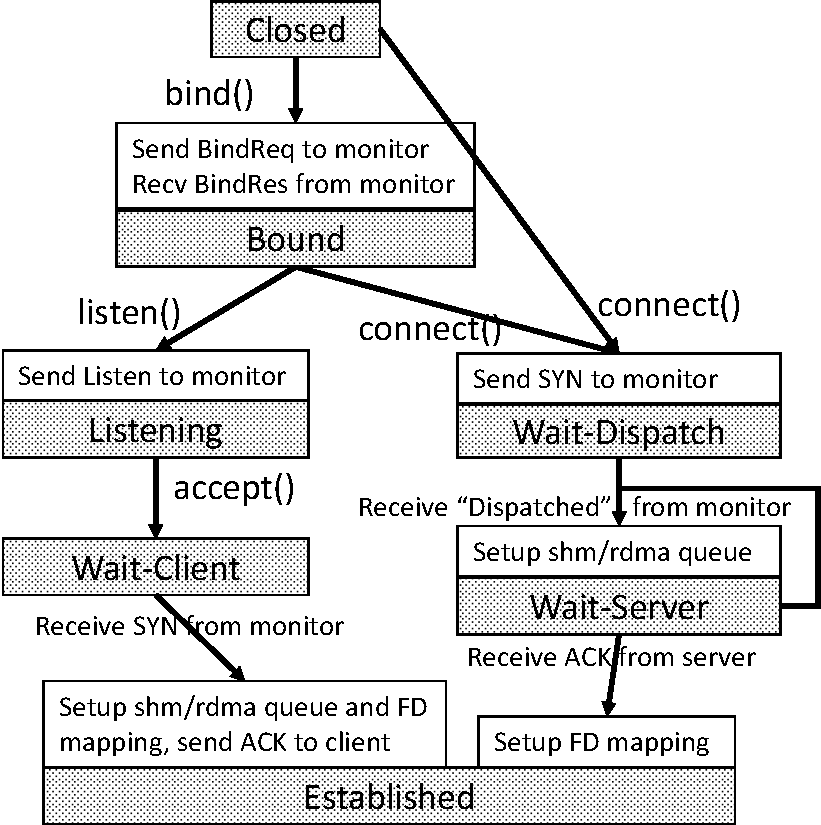
\includegraphics[width=0.3\textwidth]{images/conn-setup-new}
	\vspace{-5pt}
	\caption{State machine of connection setup in \libipc{}.}
	\label{fig:conn-setup}
\end{figure}

\parab{Dispatch new connections to listeners.}
Let's continue with the connect creation procedure assuming that both ends support \sys{}.
In Linux, new connection requests are queued in a \emph{backlog} in the kernel.
Every time the server calls \texttt{accept}, it accesses the kernel to dequeue from the backlog, which requires synchronization and adds latency.
In contrast, we maintain a per-listener backlog for every thread that listens on the socket.
The server monitor distributes SYN to a listener thread in round-robin manner.

Dispatching connection to listeners may lead to starvation when a listener does not \texttt{accept} new connections.
We devise a \textit{work stealing} approach.
When a listener invokes \texttt{accept} while the backlog is empty, it requests the monitor to steal from others' backlog.
%To avoid polling empty backlogs, each listener notifies the monitor when its backlog becomes empty.
To avoid contention between a listener and monitor, the monitor sends a request to the listener to steal from the backlog.

\parab{Establish a peer-to-peer queue.}
The first time a client and a server application communicates, the server monitor helps them establish a direct connection.
For intra-host, the monitor allocates a shared memory queue and sends the shared memory key to both client and server applications.
For inter-host, the client and server monitors establish a new RDMA QP, and send the local and remote keys to the corresponding applications.
To reduce latency, the peer-to-peer queue is established by monitor(s) when the SYN command is distributed into a listener's backlog.
However, if the SYN is stolen by another listener, a new queue needs to be established between client and the new listener, as shown in the Wait-Server state of Figure~\ref{fig:conn-setup}.

\parab{Finalize connection creation.}
After the server sets up peer-to-peer queue, as the left side of Figure~\ref{fig:conn-setup} shows, the server application sends a ACK to client application containing the client FD in SYN request and its allocated server FD.
Similar to TCP handshake, the server application can send data to the queue after sending the ACK.
When the client application receives the ACK, as shown on the right side of Figure~\ref{fig:conn-setup}, it sets up the FD mapping and can start sending data.


\begin{figure}[t!]
	\centering
	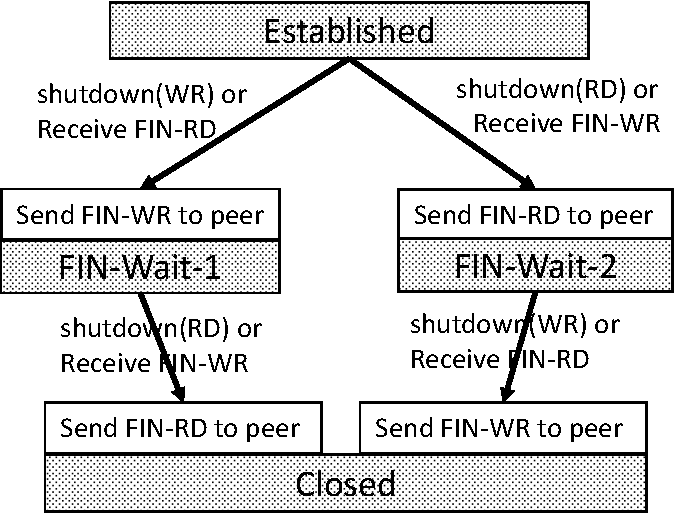
\includegraphics[width=0.25\textwidth]{images/conn-close-new}
	\vspace{-5pt}
	\caption{State machine of connection close in \libipc{}.}
	\label{fig:conn-close}
\end{figure}


\parab{Connection close.}
Closing a connection is fully peer-to-peer and does not need to involve the monitor.
Because both shared memory and RDMA are reliable and ordered communication channels, the connection close procedure is simpler than TCP.
However, we still require a handshake between peers before the FD is deleted and possibly reused by a new connection.
Otherwise, the peer might not yet have received the close message, thus sends data to the wrong connection.
Because socket is bidirectional, \texttt{close} is equivalent to \texttt{shutdown} on both send and receive directions.
As Figure~\ref{fig:conn-close} shows, when application shuts down one direction of a connection, it sends a \emph{shutdown message} to the peer.
The peer responds with a shutdown message.
A process deletes an FD when it receives shutdown messages in both directions.



\iffalse

\parab{\texttt{Bind} and \texttt{listen}.}
A \emph{server} process \texttt{bind}s a socket and needs to detect IP and port conflict. In this case, \texttt{bind} is non-partitionable and goes to the monitor. The monitor also listens on the IP and port in a user-space TCP/IP stack (\textit{e.g.} mTCP~\cite{jeong2014mtcp}, LibVMA~\cite{libvma} or Seastar~\cite{seastar}) to receive connections from other hosts.

A \emph{client} process typically \texttt{bind}s without specifying IP and port, so we need to allocate a unique IP and port for it. For scalability, we partition the loopback IP address space (127.0.0.0/8) and each process allocates IP and port in its range.

\parab{\texttt{Connect} and \texttt{accept}.}
When a client process connects to a server process on the same host, it sends a \textit{connect request} to the monitor via shared memory queue. When the server process is on another host, it creates a \textit{bootstrap TCP socket} with a special option via the user-space TCP/IP stack. If the server host supports the option, it is a \sys host and its monitor establishes an RDMA connection to the client to speedup later communications. Otherwise, the client process keeps using the bootstrap TCP socket for compatibility.

On a server host, the monitor distributes connect requests to server processes in a round-robin order, and a \textit{backlog} is maintained in each process. If the client is TCP only, the monitor proxies messages between the server process and the user-space TCP/IP stack. If the client is intra-server or RDMA capable, and it is the first time for the client and server processes to communicate, the monitor creates an inter-process queue for the process pair and sends the credentials to both processes via bootstrap sockets. After a server process \texttt{accept}s a connection in the backlog, it sends a message to the client via inter-process queue to create an FD mapping, then the socket is ready for data transmission. As Figure~\ref{fig:conn-setup} shows, connection creation takes three inter-process delays.

Distributing connection to listeners may lead to starvation when a listener does not \texttt{accept} new connections. We devise a \textit{work stealing} approach. When a listener \texttt{accept}s from empty backlog, it requests the monitor to steal from others' backlog. To avoid polling empty backlogs, each listener notifies the monitor when its backlog becomes empty. To avoid contention between a listener and monitor, the monitor sends a request to the listener rather than stealing from the backlog directly.

%\subsubsection{Connection Close}

\parab{\texttt{Close} and \texttt{shutdown}.}
Connection close is a peer-to-peer operation because only the peer process needs to be notified. If FD is deleted immediately after \texttt{close}, a new connection may reuse the FD while the peer process might not yet have received the close event thus sends data to the wrong connection. To avoid this, we require a handshake between peers.
Because socket is bidirectional, \texttt{close} is equivalent to \texttt{shutdown} on both send and receive directions.
When application shuts down one direction of a connection, it sends a \textit{shutdown message} to the peer. The peer responds with a shutdown message. A process deletes an FD when it receives shutdown messages in both directions.

%In order to achieve high scalability, we separate scalable operations to different processes. To avoid the overhead of contention, \libipc enable the file descriptor allocation by individual process and when a connection is setup, the other peer of the connection gets notified of the file descriptor number by message passing. Since we treat different threads in one process as different processes, we allocate file descriptor of different ranges to each of them to avoid collision. Since file descriptor is managed separately by each process, it is possible that a file descriptor is reused after the connection is closed. Our solution is that resources of a file descriptor is not released until an ACK is received for the close operation.

%Generally, each process in our design is treated as an endpoint in the network. Figure \ref{fig:conn-setup-close} shows the process of connection setup and close. When \textit{socket} is called, the process itself allocate per fd resources. When \textit{listen} is called, monitor is notified of port occupation. During the \textit{connect} operation, monitor first chooses one of the processes listen on this port then coordinates the creation of the shared memory between the two processes and notifies each other of the new connection. When \textit{close} happens, both of the endpoint notify each other and monitor is responsible to destroy the shared memory between them. 

\fi
